% Traceability: derived from supplement-c/examples/01_c1_solar_perihelion_native_window.tex,
% supplement-c/examples/02_c2_solar_lensing_native_window.tex,
% supplement-c/examples/03_c3_solar_redshift_native_window.tex,
% supplement-c/examples/08_c8_saturn_ring_and_moon_shell_witness.tex
\subsection{Solar system}

\subsubsection{Anomalous perihelion precession of Mercury}
\label{man:solar-perihelion-witness}
\colabbadge{manual/notebooks/04a_solar_system_mercury_perihelion.ipynb}

\begin{table}[H]
\centering
\caption{Mercury retained-extraction declaration.}
\label{tab:mercury-retention}
\begin{threeparttable}
\begin{tabularx}{\linewidth}{@{}lX@{}}
\toprule
Item & Declaration \\
\midrule
Parent field & \(\mathcal N_{\mathrm{solar}}(t_0)\) \\
Retained extraction & \(\mathcal D_{\odot,\mathrm{mercury}}\subset\mathcal N_{\mathrm{solar}}\) \\
Omitted context & remaining solar \(n\)-soma context unless declared \\
First refinement & Sun--Jupiter disoma \\
Validity window & \(100\) years, daily grid \\
Residual witness & pending until the refinement row is computed \\
\bottomrule
\end{tabularx}
\ManualTableNote{Mercury is blocked until the explicit \(\Phi_{\varpi}\) map is written.}
\end{threeparttable}
\end{table}

The cited 100-year solar-system ledger is fixed first and the perihelion witness is read as an extracted Mercury slice on that same long-window ledger.

\begin{table}[H]
\centering
\caption{Solar perihelion cited row.}
\label{tab:solar-perihelion-row}
\begin{threeparttable}
\small
\begin{tabularx}{\linewidth}{@{}lXccccc@{}}
\toprule
Row & Slice key & $T_{\mathrm{eval}}$ [\(\mathrm{bip}_0\)] & $B^*$ & $\Lambda_b$ & $R_{\mathrm{loss}}$ [\(\mathrm{trit}/\mathrm{bip}_0\)] & $T_{\mathrm{tors}}$ \\
\midrule
S1 & \texttt{tetron:*:[sun,mercury]:6} & 36525 & 137 & 6 & $\frac{1+8\ell_2}{24}$ & 3 \\
\bottomrule
\end{tabularx}
\ManualTableNote{The cited row fixes the shared long-window ledger, including the nested Earth--Moon subledger retained inside the same system ledger.}
\end{threeparttable}
\end{table}

\begin{table}[H]
\centering
\caption{Solar-system manifest on the cited 100-year ledger.}
\label{tab:solar-system-manifest}
\begin{threeparttable}
\small
\begin{tabularx}{\linewidth}{@{}lccc@{}}
\toprule
Subledger / slice & Monon-period witness & Unit & Cycle count in 100 y \\
\midrule
Mercury & 0.2408467 & y & 415.20 \\
Earth   & 1.0000174 & y & 100.00 \\
Moon    & 27.321661 & d & 1336.85 \\
Jupiter & 11.862615 & y & 8.430 \\
Saturn  & 29.447498 & y & 3.396 \\
\bottomrule
\end{tabularx}
\ManualTableNote{Mercury is the extracted perihelion slice. Earth/Moon supply the nested cadence context. Jupiter and Saturn supply the longer-window modulation context.}
\end{threeparttable}
\end{table}

\begin{table}[H]
\centering
\caption{Solar perihelion comparison attached after the cited row.}
\label{tab:solar-perihelion-comparison}
\begin{threeparttable}
\small
\begin{tabularx}{\linewidth}{@{}lcccc@{}}
\toprule
Map & Calculated [arcsec/cy] & Cited benchmark [arcsec/cy] & Abs. error [arcsec/cy] & Rel. error [\%] \\
\midrule
\(\Phi_{\varpi}\) & pending & 42.98 & pending & pending \\
\bottomrule
\end{tabularx}
\ManualTableNote{The perihelion comparison is attached only after the cited 100-year row is fixed.}
\end{threeparttable}
\end{table}

\begin{figure}[H]
\centering
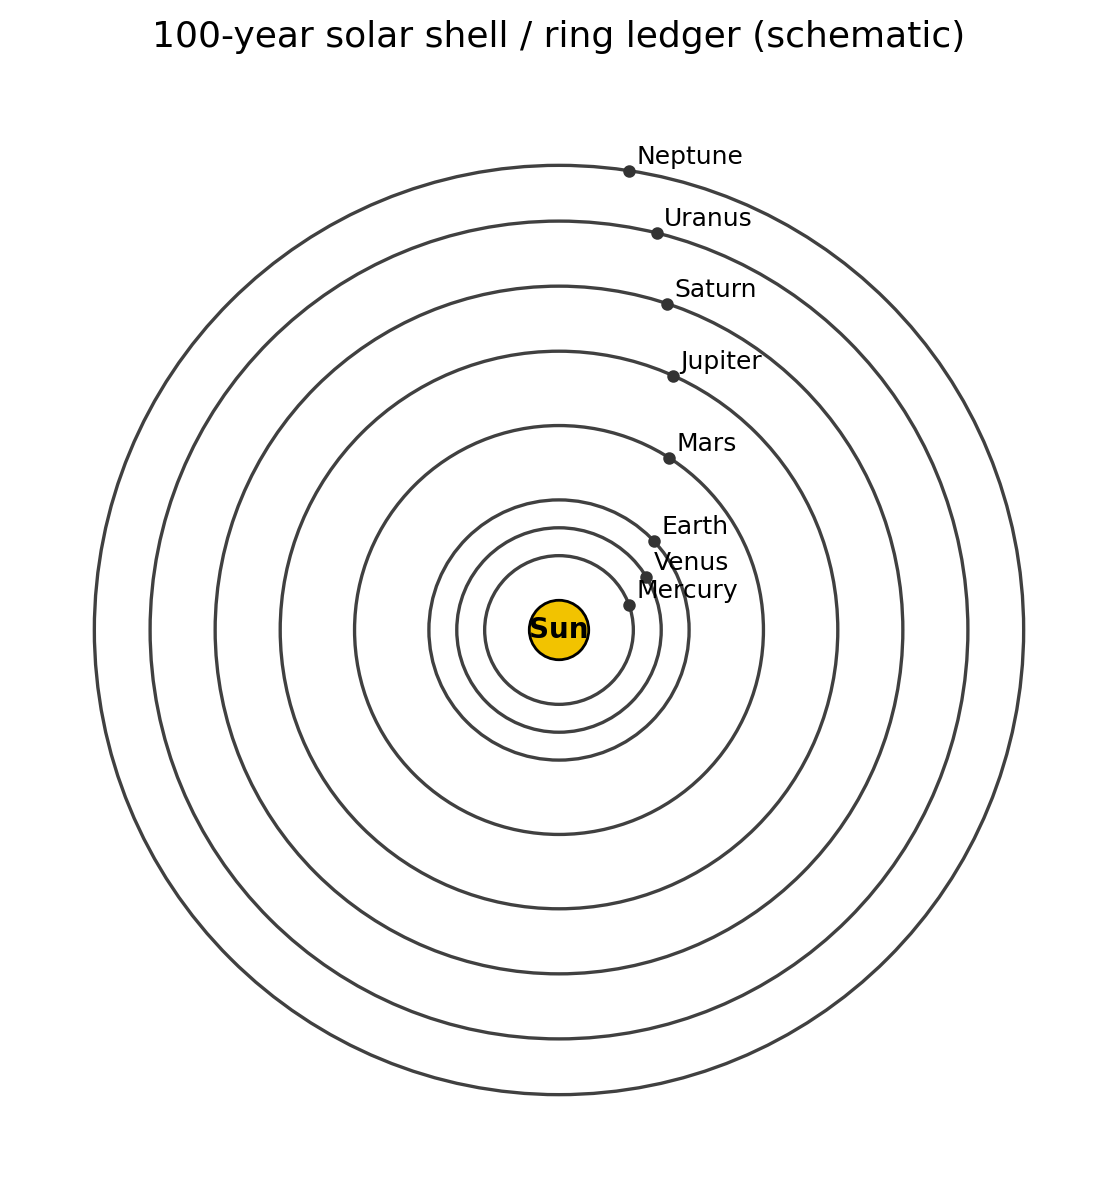
\includegraphics[width=0.72\linewidth]{figures/solar/01_system_ledger.png}
\caption{100-year solar-system ledger schematic.}
\label{fig:solar-system-ledger}
\end{figure}

\begin{figure}[H]
\centering
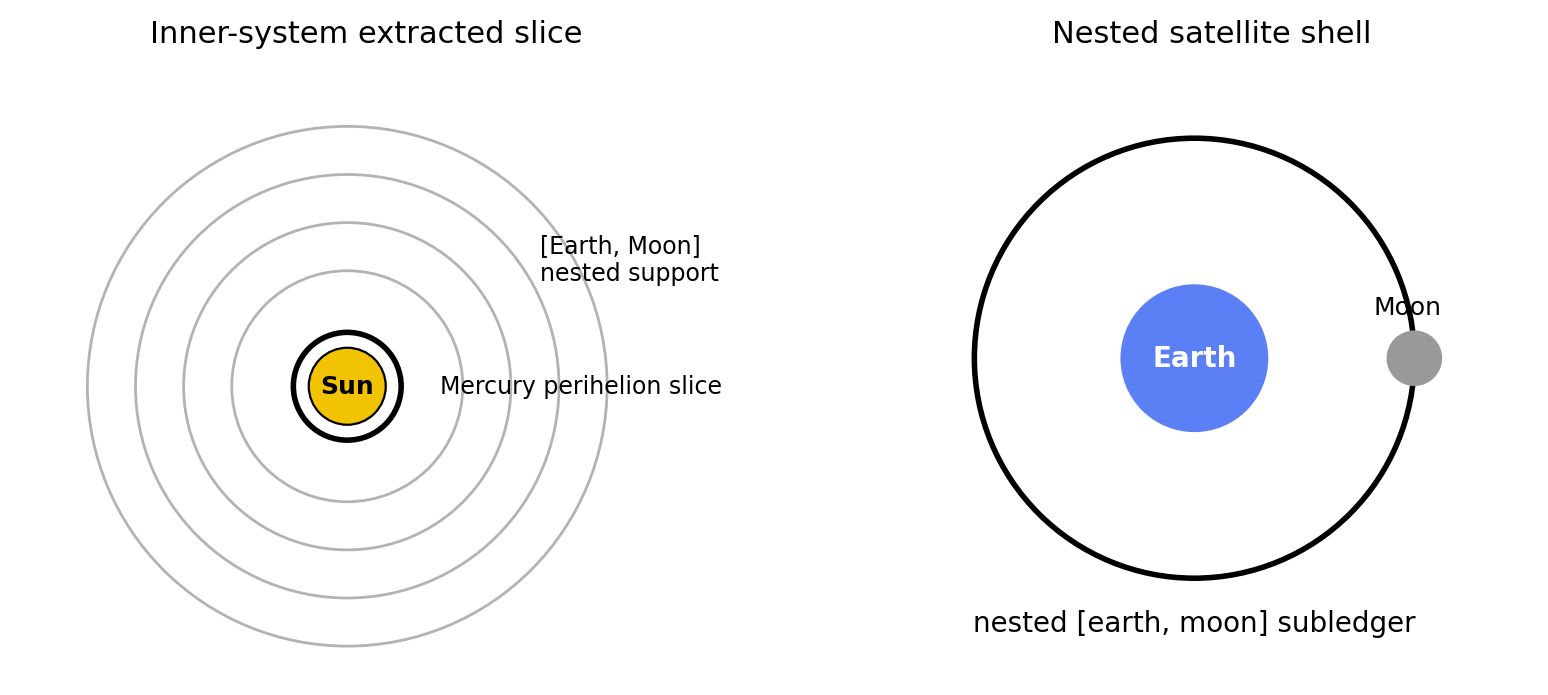
\includegraphics[width=0.88\linewidth]{figures/solar/02_mercury_earth_moon.png}
\caption{Mercury perihelion slice and nested Earth--Moon subledger.}
\label{fig:mercury-earth-moon}
\end{figure}

The long-window ledger carries the Mercury slice together with the cadence-support and residual-support witnesses of the main note.

\subsubsection{Light bending by the Sun}
\label{man:solar-lensing-witness}
\colabbadge{manual/notebooks/04a_solar_system_radiation.ipynb}

\begin{table}[H]
\centering
\caption{Solar lensing retained-extraction declaration.}
\label{tab:lensing-retention}
\begin{threeparttable}
\begin{tabularx}{\linewidth}{@{}lX@{}}
\toprule
Item & Declaration \\
\midrule
Parent field & solar export AO field \\
Retained extraction & grazing solar export slice \\
Omitted context & non-grazing solar context and external receiver details \\
First refinement & full source--receiver transfer ledger \\
Validity window & cited solar export window \\
Residual witness & pending until refinement row is computed \\
\bottomrule
\end{tabularx}
\end{threeparttable}
\end{table}

The cited solar export slice is fixed first and the grazing-incidence comparison is attached afterward.

\begin{table}[H]
\centering
\caption{Solar lensing cited row.}
\label{tab:solar-lensing-row}
\begin{threeparttable}
\small
\begin{tabularx}{\linewidth}{@{}lXcccc@{}}
\toprule
Row & Family / window & $q_{\mathrm{eff}}$ & $T_{\mathrm{tors}}$ & Packet witness & Shell qualification \\
\midrule
S2 & \texttt{duon:2:1:7} / solar export slice & $+\frac{1}{2}$ & 2 & emitted duon packet & qualified \\
\bottomrule
\end{tabularx}
\ManualTableNote{The packet witness and shell qualification are read first on the same boundary ledger.}
\end{threeparttable}
\end{table}

\begin{table}[H]
\centering
\caption{Solar lensing comparison attached after the cited row.}
\label{tab:solar-lensing-comparison}
\begin{threeparttable}
\small
\begin{tabularx}{\linewidth}{@{}lcccc@{}}
\toprule
Map & Calculated [arcsec] & Cited benchmark [arcsec] & Abs. error [arcsec] & Rel. error [\%] \\
\midrule
\(\Phi_{\mathrm{lens}}\) & pending & 1.75 & pending & pending \\
\bottomrule
\end{tabularx}
\ManualTableNote{The grazing-incidence benchmark is attached after the cited export row is fixed.}
\end{threeparttable}
\end{table}

\begin{figure}[H]
\centering
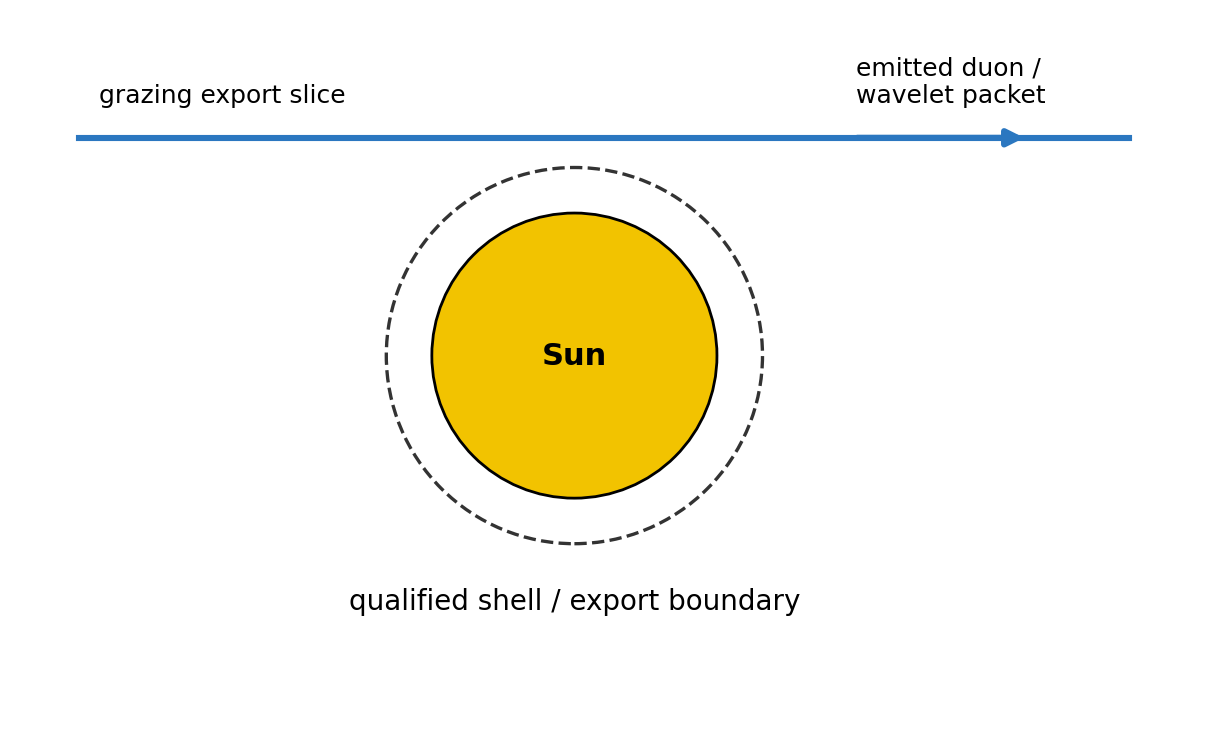
\includegraphics[width=0.72\linewidth]{figures/solar/03_lensing_export.png}
\caption{Solar lensing export witness.}
\label{fig:solar-lensing-export}
\end{figure}

The cited export ledger carries the shell/export and boundary-deflection witnesses used for the reported grazing-incidence comparison.

\subsubsection{Solar redshift}
\label{man:solar-redshift-witness}
\colabbadge{manual/notebooks/04a_solar_system_radiation.ipynb}

\begin{table}[H]
\centering
\caption{Solar redshift retained-extraction declaration.}
\label{tab:redshift-retention}
\begin{threeparttable}
\begin{tabularx}{\linewidth}{@{}lX@{}}
\toprule
Item & Declaration \\
\midrule
Parent field & solar transfer AO field \\
Retained extraction & source--receiver transfer pair \\
Omitted context & external transfer windows not declared in the pair \\
First refinement & multi-window transfer ledger \\
Validity window & cited source/receiver windows \\
Residual witness & pending until refinement row is computed \\
\bottomrule
\end{tabularx}
\end{threeparttable}
\end{table}

The cited source and receiver windows are fixed first and the redshift comparison is attached afterward as a two-window transfer witness.

\begin{table}[H]
\centering
\caption{Solar redshift cited row.}
\label{tab:solar-redshift-row}
\begin{threeparttable}
\small
\begin{tabularx}{\linewidth}{@{}lXcc@{}}
\toprule
Row & Transfer class & $B^*$ & $\Lambda_b$ \\
\midrule
S3 & \texttt{duon:2:1:7} on the transfer class & 137 & 6 \\
\bottomrule
\end{tabularx}
\ManualTableNote{The source and receiver rows are fixed first. The burden difference and cadence-transfer comparison are attached afterward across the same two-window ledger.}
\end{threeparttable}
\end{table}

\begin{table}[H]
\centering
\caption{Solar redshift comparison attached after the cited rows.}
\label{tab:solar-redshift-comparison}
\begin{threeparttable}
\small
\begin{tabularx}{\linewidth}{@{}lcccc@{}}
\toprule
Map & Calculated & Cited benchmark & Abs. error & Rel. error [\%] \\
\midrule
\(\Phi_z\) & pending & $2.12\times10^{-6}$ & pending & pending \\
\bottomrule
\end{tabularx}
\ManualTableNote{The redshift witness is attached after the source and receiver rows are fixed on the same two-window ledger.}
\end{threeparttable}
\end{table}

\begin{figure}[H]
\centering
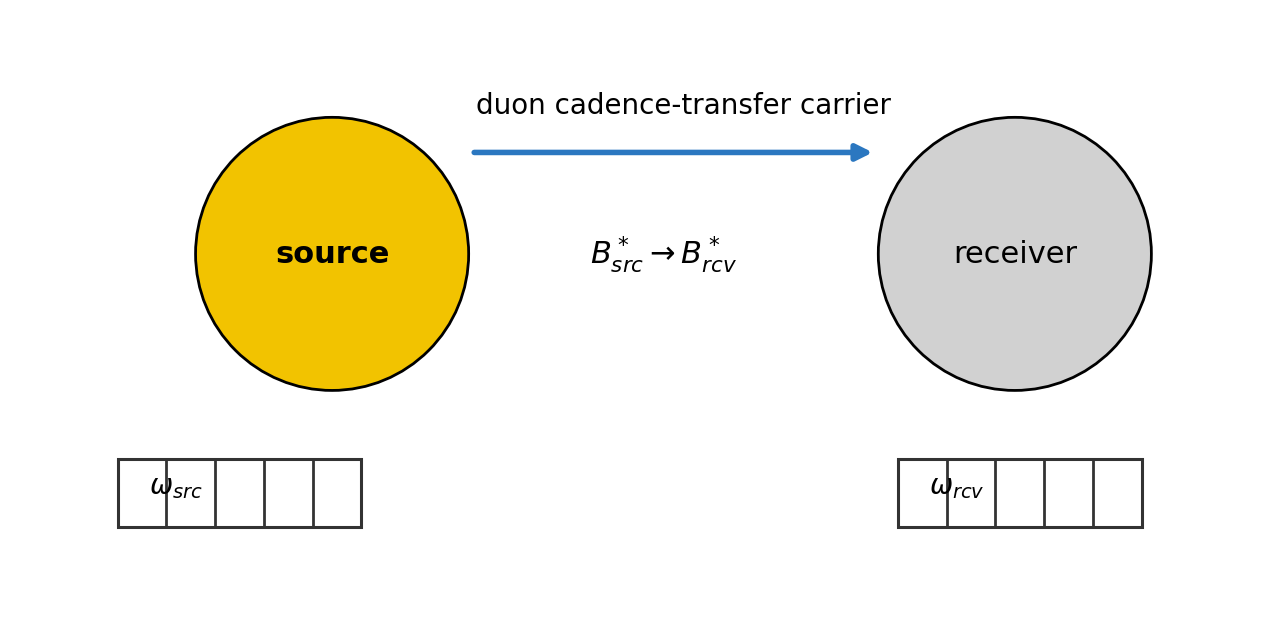
\includegraphics[width=0.72\linewidth]{figures/solar/04_redshift_transfer.png}
\caption{Solar redshift transfer witness.}
\label{fig:solar-redshift-transfer}
\end{figure}

The two-window ledger carries the cadence-transfer witness used for the reported redshift comparison.

\subsubsection{Saturn rings and moon shells}
\label{man:saturn-shell-witness}
\colabbadge{manual/notebooks/04a_solar_system_saturn.ipynb}

\begin{table}[H]
\centering
\caption{Saturn retained-extraction declaration.}
\label{tab:saturn-retention}
\begin{threeparttable}
\begin{tabularx}{\linewidth}{@{}lX@{}}
\toprule
Item & Declaration \\
\midrule
Parent field & solar \(n\)-soma orbital ledger \\
Retained extraction & Saturn ring--moon shell family \\
Omitted context & non-Saturn solar context \\
First refinement & outer solar shell-family ledger \\
Validity window & cited Saturn orbital shell window \\
Residual witness & qualitative until refinement row is computed \\
\bottomrule
\end{tabularx}
\end{threeparttable}
\end{table}

The cited Saturn ring family and selected moon shells are fixed first and then reported as one shell-family witness.

\begin{table}[H]
\centering
\caption{Saturn ring-and-moon cited row.}
\label{tab:saturn-shell-row}
\begin{threeparttable}
\small
\begin{tabularx}{\linewidth}{@{}lXc@{}}
\toprule
Row & Structural key & Gap witness \\
\midrule
S4 & \texttt{tetron:*:[saturn,rings]:6} & Cassini Division \\
\bottomrule
\end{tabularx}
\ManualTableNote{The cited row records the shell family and the Cassini Division gap on the same ordered orbital ledger.}
\end{threeparttable}
\end{table}

\begin{table}[H]
\centering
\caption{Saturn ring family and selected moons.}
\label{tab:saturn-shell-family}
\begin{threeparttable}
\small
\begin{tabularx}{\linewidth}{@{}lcc@{}}
\toprule
Band / moon & Radius witness [km] & Period witness [d] \\
\midrule
D--E ring family & --- & --- \\
Mimas & 185{,}539 & 0.942 \\
Enceladus & 237{,}948 & 1.370 \\
Tethys & 294{,}619 & 1.888 \\
Dione & 377{,}396 & 2.737 \\
Rhea & 527{,}069 & 4.518 \\
Titan & 1{,}221{,}870 & 15.945 \\
\bottomrule
\end{tabularx}
\ManualTableNote{The D--E ring family is the inner ring witness. The selected moons supply the outer shell cadence, with Titan as the slow outer shell witness.}
\end{threeparttable}
\end{table}

\begin{figure}[H]
\centering
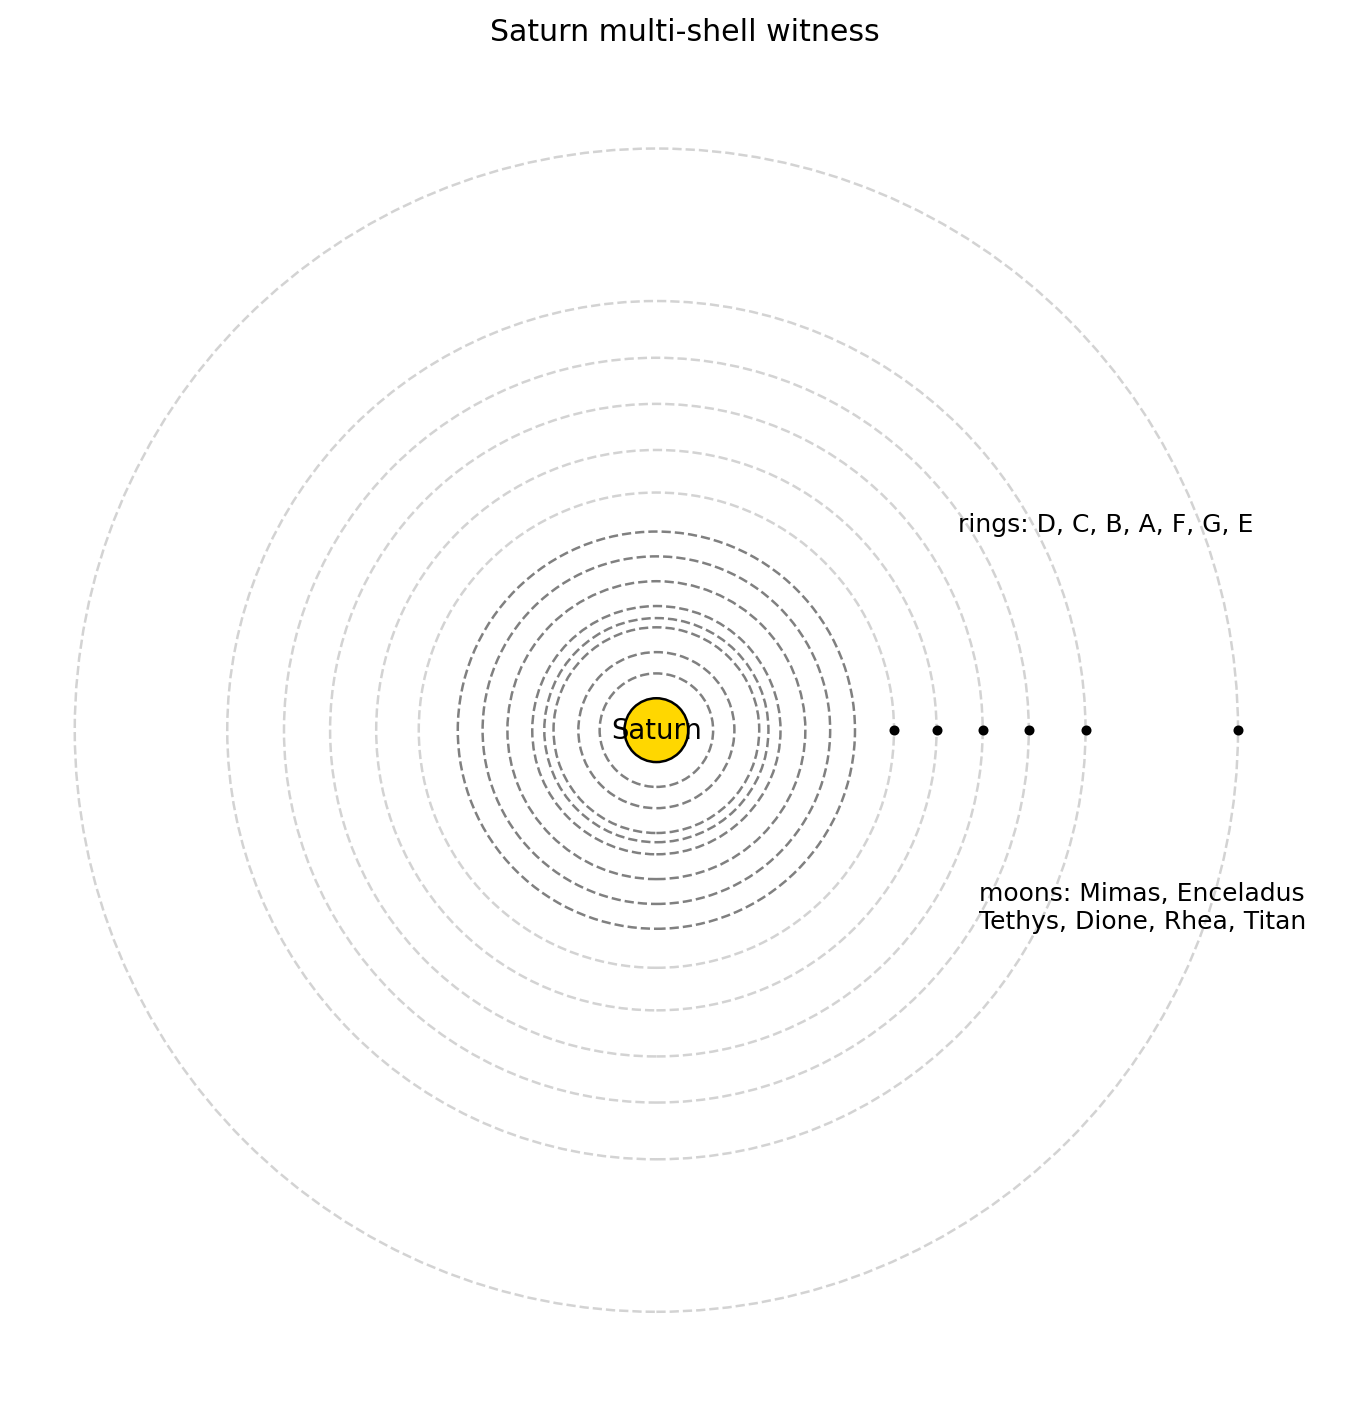
\includegraphics[width=0.74\linewidth]{figures/saturn/01_saturn_shell_family.png}
\caption{Saturn rings and selected moons as a multi-shell witness.}
\label{fig:saturn-shell-family}
\end{figure}

The ring family and selected moons display a readable multi-shell witness on the same orbital ledger.
